\documentclass[12pt]{article}
\usepackage{graphicx}
\usepackage{epstopdf}
\usepackage[spanish]{babel}
\selectlanguage{spanish}
%\usepackage[english]{babel}
\usepackage[utf8]{inputenc}
\usepackage{hyperref}
\usepackage[left=3cm,top=3cm,right=3cm,bottom= 2.5cm,nohead,nofoot]{geometry}
\usepackage{braket}
\usepackage{datenumber}
\usepackage{textcomp}
\usepackage{chemfig}%figuras Quimica
\usepackage[version=4]{mhchem}%nombres compuestos quimicos
%\newdate{date}{10}{05}{2013}
%\date{\displaydate{date}}

\begin{document}

\begin{center}
%\Huge
\LARGE
Simulaciones por Din\'{a}mica Molecular para el Estudio de Propiedades Biof\'{i}sicas de Estafiloxantina en Membranas Modelo de \textit{Staphylococcus aureus}\\
\vspace{3mm}
\large
John Erick Cabrera Ramirez 

%\large
 C\'odigo: 201823444


\vspace{2mm}
\large
Directores: Chad Leidy (Departamento
de física) y Camilo Aponte-Santamaría (Grupo tándem Max Planck de biofísica computacional, MPTG-CBP)

\normalsize
\vspace{2mm}

\today
\end{center}


\normalsize
\tableofcontents
\newpage
\begin{abstract}
\textit{Staphylococcus aureus} es un patógeno de importancia clínica que ha recibido gran atención pública debido al desarrollo de resistencia a diferentes antibióticos tradicionales dirigidos a inhibir la síntesis de la pared de péptidoglicando que recubre la bacteria. Como alternativa de tratamiento se está estudiando el mecanismo de acción de los péptidos antimicrobianos dirigidos a comprometer la integridad de la membrana lipídica de la bacteria. Los péptidos antimicrobianos atacan a la membrana plasmática de la bacteria formando poros, los cuales disipan el potencial electroquímico requerido para mantener viva la bacteria. Es importante estudiar las propiedades mecánicas de la membrana plasmática ya que la bacteria puede modular estas propiedades a través de cambios en su composición lipídica, lo cual puede resultar en incrementos en resistencia a péptidos antimicrobiales. Uno de los compuestos que se ha estudiado en \textit{Staphylococcus aureus} es  el carotenoide estafiloxantina, el cual aumenta  su concentración en la membrana plasmática cuando la bacteria está sometida a estrés. Algunos estudios han sugerido que el papel de este carotenoide es aumentar la rigidez de la membrana plasmática de la bacteria. Sin embargo, aún no está clara la función que cumple en la membrana asociada a sus propiedades biofísicas locales, propiedades tales como la orientación y las interacciones con lípidos cercanos. Uno de los métodos que puede contribuir al estudio del papel local de la estafiloxantina en la membrana es el de las simulaciones por dinámica molecular. En estas simulaciones se simula la trayectoria de los átomos que conforman cada molécula de un fragmento pequeño (128 lípidos y sus moléculas de agua asociadas) de la membrana plasmática.
Debido al vacío existente en el conocimiento de estafiloxantina en \textit{Staphylococcus aureus} es objeto del presente trabajo estudiar el rol mecánico de la estafiloxantina al insertarse en dos membranas modelo de \textit{Staphylococcus aureus}: una que contiene DMPG y otra que contiene DPPG. El rol mecánico de la membrana se estudiará mediante sumulaciones por dinámica molecular en las cuales se usarán los campos de fuerza de AMBER y de CHARMM. En estos campos se optimizarán los parámetros de los ángulos dihedros de los diferentes grupos moleculares de estafiloxantina para tratar de reflejar el comportamiento físico de la molécula. De las simulaciones se pueden obtener propiedades biofísicas como el parámetro de orden del deuterio, la orientación de la estafiloxantina, el área por lípido, entre otras. Estas propiedades pueden ser utilizadas para predecir cambios en las propiedades mecánicas de la membrana en presencia de esta molécula.

\end{abstract}
\newpage
\section{Introducci\'on}

\textit{Staphylococcus aureus} es una bacteria pat\'{o}gena Gram Positiva que causa enfermedades infecciosas. De acuerdo a Kobayashi et al. \cite{Kobayashi2015PathogenesisAbscesses}, la bacteria es un colonizador común de la piel y del aparato respiratorio y actúa como un patógeno oportunista que puede causar infecciones nicosomiales (intrahospitalarias) en el sistema respiratorio, en los tejidos blandos y en el torrente sangu\'ineo \cite{HarpavatS.NissimS.LipppincottsMicrocards:MicrobiologyFlashCards2012.}. Incluso puede causar infecciones en las junturas de las pr\'otesis formando biopel\'iculas \cite{Meylan2018}.\\

%En la figura \ref{fig:sta} se muestra una microfotograf\'ia de \textit{Staphylococcus aureus} resistente a antibi\'oticos.\\

%\begin{figure}[h]
%\begin{center}
 % 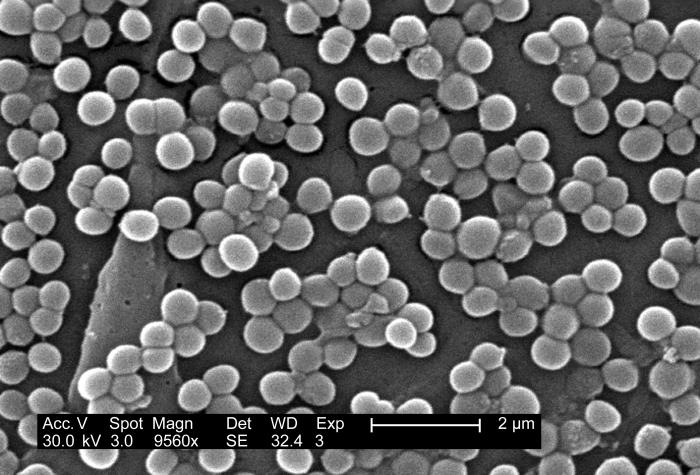
\includegraphics[scale=0.3]{saureus.jpg}
  %\caption{Imagen  de \textit{Staphylococcus aureus} obtenida con un microscopio electr\'onico de barrido (SEM). Tomado de \cite{HaneyCar2005PublicAureus}.}
  %\label{fig:sta}
%\end{center}
%\end{figure}

Desde el descubrimiento de \textit{Staphylococcus aureus} como causante de una infecci\'on a una herida en 1881 \cite{Orent2006AMagazine} se ha investigado su presencia en otras infecciones y se han utilizado antibi\'oticos como la penicilina, la meticilina y la vancomicina para controlar estas infecciones   \cite{HarpavatS.NissimS.LipppincottsMicrocards:MicrobiologyFlashCards2012.}. No obstante, \textit{Staphylococcus aureus} ha desarrollado resistencia a algunos de estos antibi\'oticos,  de ahí que surja la necesidad de buscar nuevos antibi\'oticos o incluso moléculas con un mecanismo de acción diferente. Una posible familia de moléculas que podrían actuar como alternativas serían los péptidos antimicrobianos (estos se describen en la sección \ref{ss:anti}).\\

De acuerdo a Perez-Lopez et al. \cite{Perez-LopezVariationsProperties} y Nagendra et al.  \cite{Nagendra2011} se ha encontrado que la bacteria modula la composición de su membrana plasmática frente a cambios en el medio. Esta modulación afecta las propiedades biofísicas de su membrana, es decir propiedades fisicoquímicas como la permeabilidad, la estructura y las propiedades mecánicas. El cambio de estas propiedades es un factor que mejora la tolerancia de la bacteria a la acción de péptidos antimicrobiales. Debido a esto, las propiedades biofísicas de la membrana se convierten en objeto de estudio y además son determinantes en la búsqueda de nuevas moléculas dirigidas a la membrana (moléculas blanco) que combatan la bacteria. \\

Al ser \textit{Staphylococcus aureus}\footnote{\textit{Staphylococcus aureus} al ser una bacteria Gram positiva está envuelta por una  membrana llamada bicapa lipídica y recubierta de una pared externa de péptidoglicando. Las membranas se explican en la subsección \ref{ss:mem}} una bacteria Gram positiva, consta de una membrana plasmática que es de interés en términos de la generación de nuevos antibióticos antimicrobiales debido a su rol como mediador del potencial electroquímico. Algunos estudios se han enfocado en cómo la composición de la bicapa lipídica interna afecta sus propiedades biofísicas con base en cambios en la concentración de ciertos lípidos como la cardiolipina \cite{Hernandez-Villa1BiophysicalPeptides} y de carotenoides como la estafiloxantina \cite{MelendezDelgado2018StudyingBilayers}, \cite{Perez-LopezVariationsProperties}, \cite{Nagendra2011}. Recientemente, en nuestros grupos, se han estudiado computacionalmente y experimentalmente propiedades mecánicas como la rigidez de la membrana, la orientación de la estafiloxantina, el área por lípido, la difusión y el parámetro de orden del deuterio de diferentes membranas modelo.\\

En los experimentos realizados por Perez-Lopez et al. \cite{Perez-LopezVariationsProperties} y Nagendra et al.  \cite{Nagendra2011} se ha mostrado que cambios en el contenido de carotenoides en las membranas, en diferentes etapas de crecimiento \textit{Staphylococcus aureus}, y en membranas modelo compuestas por algunos lípidos mayoritarios de la bacteria, resultan en cambios en la rigidez. Se ha demostrado que este cambio en rigidez afecta la resistencia de la membrana a diferentes péptidos antimicrobiales. Sin embargo, es necesario mirar a nivel molecular la influencia local que tienen los carotenoides en la membrana para entender como la presencia de estas moléculas puede influir en las propiedades mecánicas. Debido a su resolución, los experimentos realizados no permiten vislumbrar diferentes propiedades moleculares que puedan explicar este fenómeno. Alternativamente, las simulaciones de dinámica molecular (MD por sus siglas en inglés) si permiten hacer este acercamiento. La MD se ha convertido en una herramienta excelente para estudiar membranas biológicas \cite{Marrink2019ComputationalMembranes}. Este método monitorea la evolución espacio-temporal de sistemas biológicos a una escala atómica y asi permite determinar información estructural (termo)dinámica y energética de membranas, que complementa y expande las técnicas experimentales. 
Entre las propiedades que se pueden estudiar en detalle a través de simulaciones están la ubicación relativa de los carotenoides con respecto a los otros lípidos, la orientación y las interacciones que presenta exclusivamente el carotenoide estafiloxantina con los lípidos vecinos. Estos detalles moleculares influyen en los cambios de la rigidez de la membrana de \textit{Staphylococcus aureus}.\\

Para estudiar la ubicación, las interacciones con otros lípidos, el área por lípido,  de la estafiloxantina, en nuestro grupo se ha realizado un estudio computacional preeliminar mediante las simulaciones por dinámica molecular  implementadas en CHARMM \cite{MelendezDelgado2018StudyingBilayers}  (ver sección \ref{ss:pre}). Estas simulaciones requieren introducir ciertos parámetros relacionados con los campos de fuerza y con la geometría de la estafiloxantina, los cuales deben ser cuidadosamente seleccionados para que las simulaciones por dinámica molecular reflejen el comportamiento físico de la molécula.\\

En una aproximación inicial, Meléndez et al. \cite{MelendezDelgado2018StudyingBilayers} utilizaron el protocolo implementado en CHARMM-GUI \cite{Sunhwan2008CHARMM-GUI:CHARMM} para determinar los parámetros de estafiloxantina. Algunos de los parámetros obtenidos a través de este procedimiento para la estafiloxantina no se han optimizado completamente. El objetivo de la  presente propuesta es optimizar los parámetros generados por CHARMM-GUI para la estafiloxantina, para que luego puedan ser utilizados en simulaciones MD a la luz del trabajo previo realizado \cite{MelendezDelgado2018StudyingBilayers}. Adicionalmente, proponemos modelar la estafiloxantina utilizando un segundo campo de fuerzas (llamado AMBER). Éste modelamiento nos permitirá estudiar la dinámica de bicapas lipídicas en presencia de estafiloxantina y confirmar que las observaciones que hagamos sean independientes del potencial de fuerzas utilizado.\\


\section{Estado del Arte}
\subsection{La membrana Bacteriana y sus compuestos presentes}\label{ss:mem}
Según el tipo de membrana que posean las bacterias, estás pueden clasificarse en dos grandes clases: las bacterias Gram positivas y las bacterias Gram negativas. Las bacterias Gram positivas poseen una sola bicapa lipídica envuelta en una capa compuesta por unos polímeros de azúcares y aminoácidos llamados peptidoglicando (ver figura \ref{fig:mem}), mientras que las membranas de bacterias Gram negativa poseen dos bicapas lipídicas. Ya que \textit{Staphylococcus aureus} es una bacteria Gram positiva se discutirá principalmente la composición de la membrana de las bacterias Gram Positivas.\\

\begin{figure}[h]
\begin{center}
  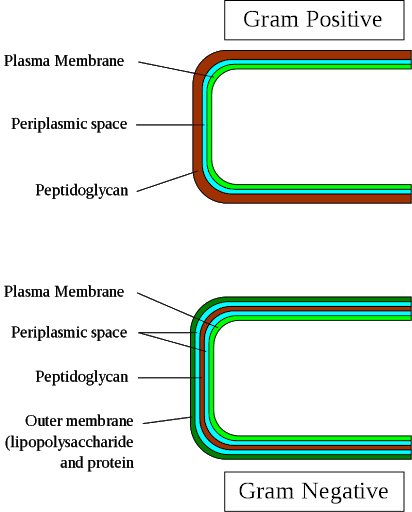
\includegraphics[scale=0.3]{grampos1.png}
    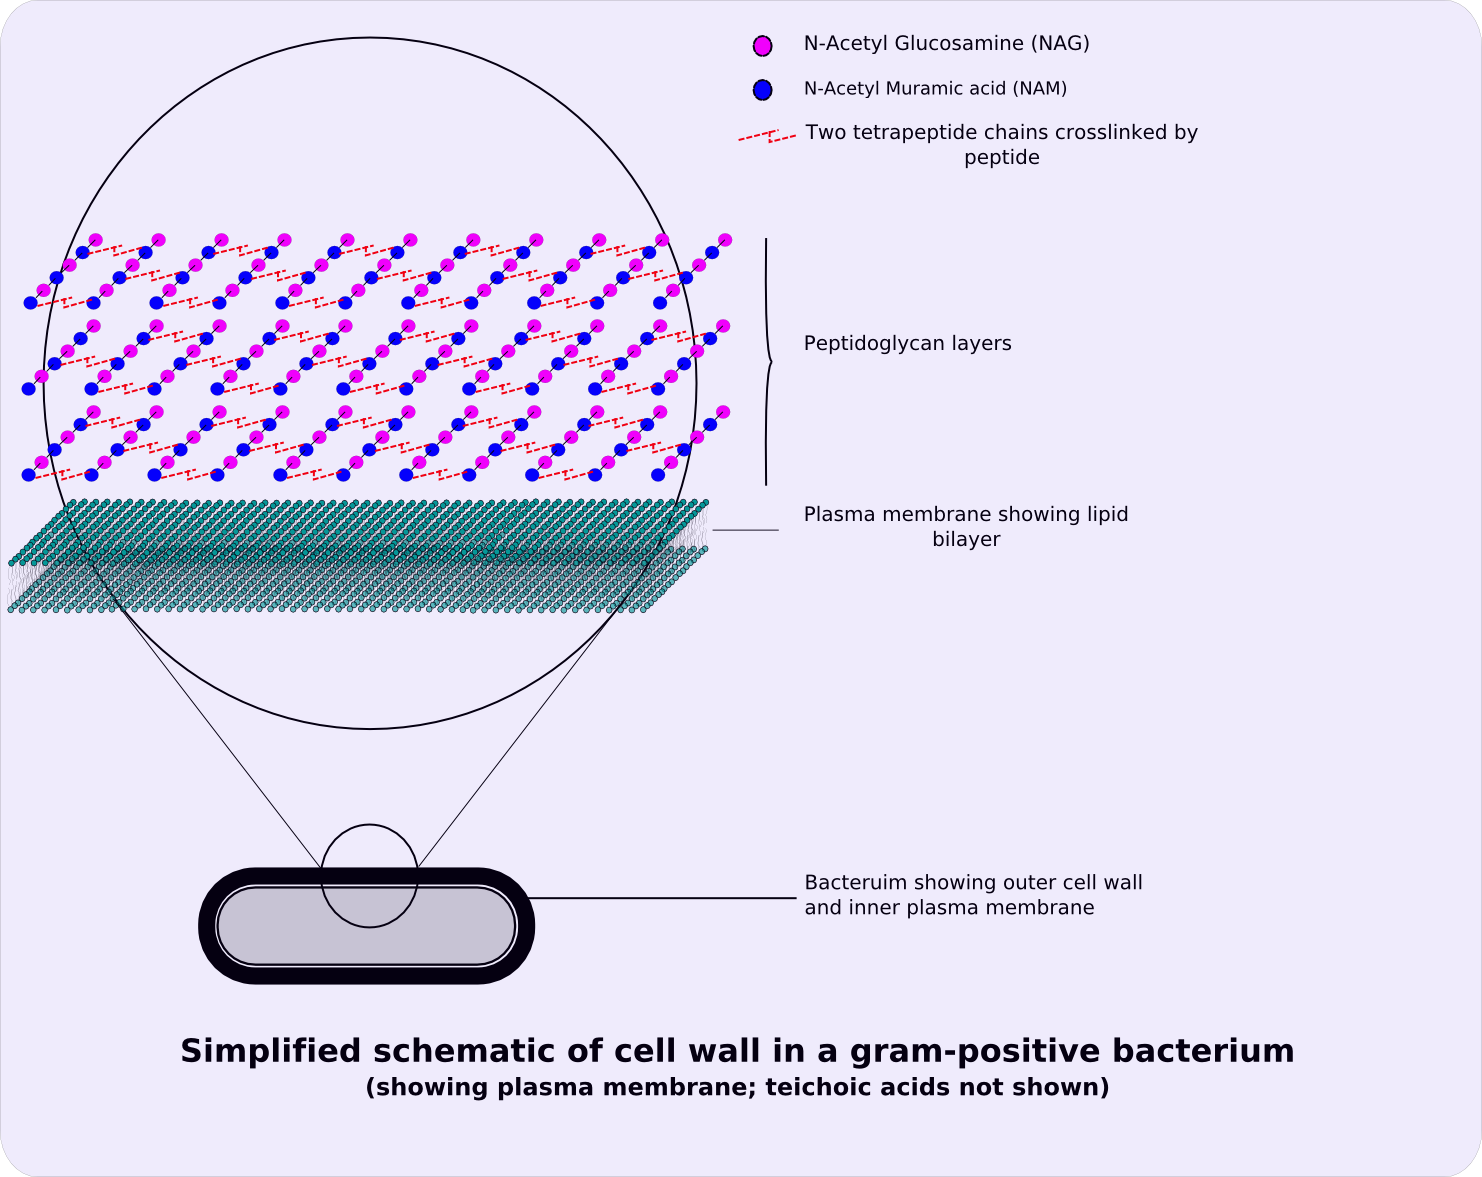
\includegraphics[scale=0.15]{grampos2.png}
  \caption{Imagen  de la membrana de una bacteria Gram positiva. Tomado de \cite{Nelson2011}.}
  \label{fig:mem}
\end{center}
\end{figure}
La bicapa lipídica es una membrana presente en todos las células la cual está compuesta mayoritariamente por lípidos. Los lípidos se acomodan de tal manera que el espesor de la membrana sea de dos lípidos de grosor. En su mayoría, con excepciones como los esteroles, los lípidos están compuestos por una o varias cadenas de ácidos grasos no polares (cadenas hidrocarbonadas con carboxilo) unidas a diferentes sustituyentes polares los cuales pueden presentar carga o no a pH fisiológico. De acuerdo a los sustituyentes y al tipo de ácidos grasos, cada lípido presenta propiedades fisicoquímicas específicas como la carga total, la polaridad, y el largo que lo distinguen a nivel biofísico con los otros lípidos. Los lípidos forman bicapas debido a la presencia del agua ya que al ser moléculas anfipáticas (combinando motivos polares y apolares) se orientan con respecto a esta. La parte hidrofílica del lípido interactúa con el agua mientras que la parte hidrofóbica no interactúa con esta, lo que induce reorientación y agregación de los lípidos. Estas interacciones hacen que sea más estable encontrar los lípidos inmersos en el agua formando agregados sin mezclarse con el agua. La interacci\'on lateral entre estas mol\'eculas se da a trav\'es de fuerzas no covalentes lo que le confiere propiedades de cristal l\'iquido caracterizado por la capacidad de presentar transiciones de fase s\'olido-l\'iquido y difusión lateral. \\

La bicapa lipídica de \textit{Staphylococcus aureus} esta compuesta principalmente por fosfatidilgliceroles (PG), cardiolipina (CL), lifosfoglicandos (LPG) y glicopeptidolípidos (GPL) \cite{Sohlenkamp2015BacterialPathways}. En la figura \ref{fig:DMPG} se muestra la fórmula estructural del Dimiristoilfosphatidilglicerol (DMPG), el cual es un lípido con el fosfatidilglicerol unido a dos miristoil (provenientes del ácido mirístico). 
\\

\begin{figure}[h]
\begin{center}
    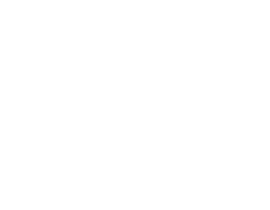
\includegraphics[scale=0.4]{DMPG.png}
  \caption{Fórmula estructural del Dimiristoilfosphatidilglicerol (DMPG). Tomada de \cite{CHEMDRUGDMPGDimyristoylphosphatidylglycerol}.}
  \label{fig:DMPG}
\end{center}
\end{figure}
Las membranas lipídicas además de tener lípidos contienen otros tipos de biomoléculas como los carotenoides, las proteínas y los glicolípidos que tienen relevancia fisiológica en la célula. Los carotenoides en particular pigmentan las células. En el caso de \textit{Staphylococcus aureus} se ha descubierto que los carotenoides juegan un papel importante en la integridad de la membrana celular y protegen a la bacteria frente a estrés oxidativo \cite{Nagendra2011}. La protección de los carotenoides en la membrana se ve reflejada por un aumento de su rigidez, de forma similar al papel que juega el colesterol en la membrana eucariótica. \\

Uno de los carotenoides más relevantes en \textit{Staphylococcus aureus} es la estafiloxantina la cual le da el nombre a la bacteria ya que le da un color aúreo. La estafiloxantina es un  triterpeno carotenoide que posee dos cadenas hidrocarbonadas. Una de ellas es un ácido graso parecido a otros acidos grasos de la membrana, caracterizado por ser saturado y con presencia de ramificaciones metiles. El otro es un ácido graso diaponeurosporenoico, que presenta insaturaciones conjugadas tipo trans y ramificaciones.  Las dos cadenas están unidas a un molécula de glucosa mediante enlaces tipo éster, ver figura \ref{fig:stx}. Debido a los enlaces dobles conjugados de la cadena diaponeurosporenoica, esta es rígida, ya que estos enlaces dificultan rotaciones intramoleculares. Esta rigidez se convierte en un factor que aumenta el empaquetado de la bicapa lípídica, ya que disminuye la distancia entre lípidos vecinos \cite{Heimburg}.\\

\begin{figure}[h]
\begin{center}
  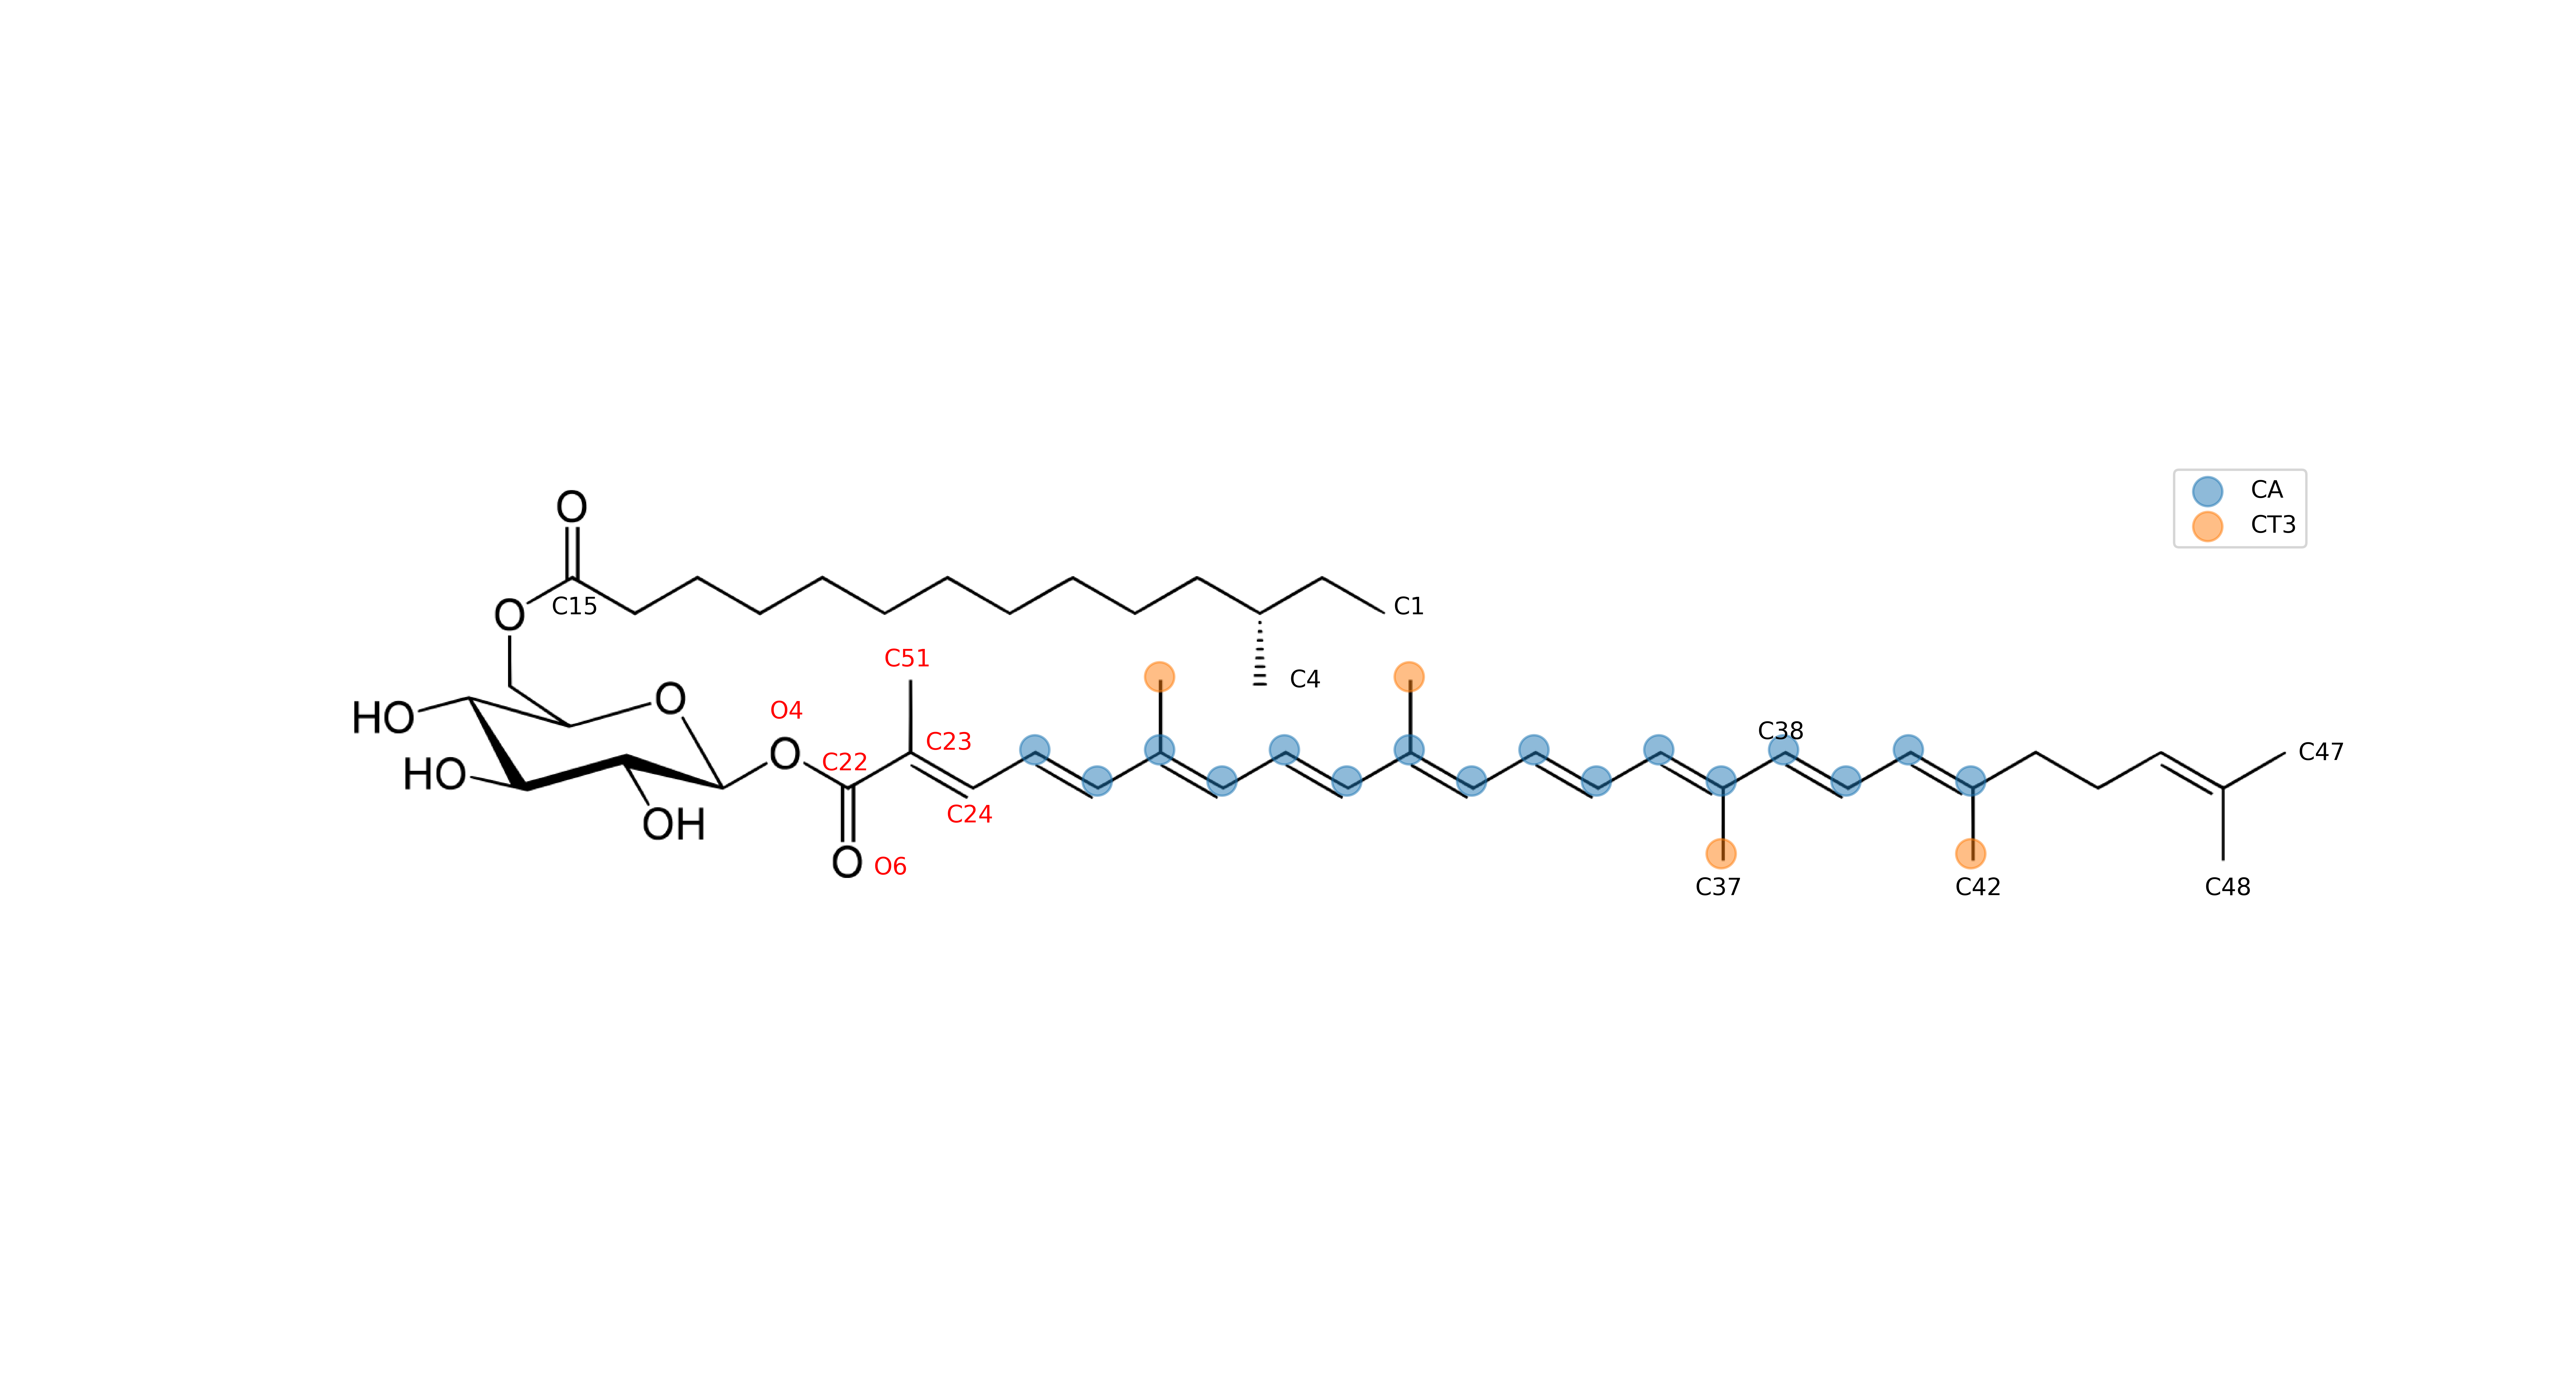
\includegraphics[scale=0.4]{stx_problems.png}
  \caption{Fórmula estructural de la estafiloxantina. Tomada de \cite{MelendezDelgado2018StudyingBilayers}.}
  \label{fig:stx}
\end{center}
\end{figure}
 Adem\'{a}s, estas insaturaciones conjugadas le dan propiedades antioxidantes que protegen a la bacteria frente al estrés oxidativo del medio, al poder incorporar especies reactivas oxidativas \cite{Nelson2011}.
\subsection{Resistencia a tratamientos antibióticos de \textit{Staphylococcus aureus}}\label{ss:anti}
Desde el descubrimiento de la penicilina, infecciones de \textit{Staphylococcus aureus} han sido tratadas con este antibiótico. Sin embargo, a mediados del siglo XX \textit{Staphylococcus aureus} comenzó a presentar resistencia a esta familia de antibióticos $\beta$-lactámicos, incluida la meticilina. Posteriormente se han aplicado otros antibióticos como la vancomicina, pero también se ha ido generando  resistencia a estos otros antibióticos.  De la resistencia a antibióticos surge la necesidad de buscar nuevos medicamentos que combatan \textit{S. aureus}.\\

Un p\'eptido antimicrobiano es  un olig\'omero de amino\'acidos, de alrededor de 20 aminoacidos de largo, que hace parte de la respuesta inmune de un amplio espectro de especies, y que son faciles de sintetizar en el laboratorio. Los péptidos antimicrobianos se clasifican según la estructura secundaria que tienen: $\alpha$ h\'elices, $\beta$ plegados.   Los p\'eptidos antimicrobianos interact\'uan con la membrana de la bacteria produciendo orificios que causan p\'erdida de contenido, pérdida del potencial electroquímico y muerte celular.\\

Los péptidos antimicrobiales forman estructuras anfipáticas que inducen su adhesión a la membrana. Al aumentar su concentración superficial, se induce una inserción de estos péptidos, atravesando la membrana y generando poros. Son de interés los péptidos antimicrobiales catiónicos ya que la membrana de \textit{Staphylococcus aureus} es aniónica y estos péptidos tienen una preferencia para adherirse a estas membranas. La formación de poros es un proceso mecánico que requiere la deformación de la membrana para suceder. Al incrementar la rigidez de la membrana, se dificulta la inserción del péptido generando resitencia \cite{Perez-LopezVariationsProperties}, \cite{Nagendra2011}. Por este motivo se vuelve relevante estudiar como la composición de la membrana, en particular la presencia de stafiloxantina, modula la rigidez de la membrana.
\subsection{Dinámica Molecular y Campos de Fuerza}\label{ss:md} 
Un paradigma central en la biología es la existencia de un vínculo entre la secuencia, la estructura, la dinámica y la función de una biomolécula, entiéndase esta última como cualquier molécula con un rol biológico \cite{Cui2006}. No únicamente la secuencia de aminoácidos o secuencia de nucleóticos, sino también la estructura y a la dinámica son determinantes en la función de cualquier biomolécula. En el caso de las membranas biológicas, la complejidad aumenta, ya que a las proteínas de membrana, que se encargan de diversas funciones fisiológicas para las células y sus organelos, se suma una rica composición de lípidos. Los lípidos no son entes pasivos que proveen un medio bidimensional para las proteínas de membrana. Por el contrario, ellos afectan tanto las propiedades bioquímicas como las propiedades físicas, como la movilidad y la rigidez de las membranas y así en últimas influir en su función.\\

Un método poderoso para estudiar la dinámica de biomoléculas, y en particular las membranas biológicas, es el de las simulaciones por dinámica molecular (MD por sus siglas en inglés).\\

En la dinámica molecular se resuelven numéricamente las ecuaciones de movimiento de Newton para cada una de las partículas que constituyen el sistema, por ejemplo a nivel de átomos (alta resolución espacial) o grupos de atomos (menor resolución espacial), de donde se obtiene la trayectoria en función del tiempo de cada partícula. Una vez obtenida la trayectoria se pueden analizar las propiedades del sistema en estudio, a partir las velocidades, posiciones y energías de interacción de todo el sistema, registradas durante la simulación.\\

Las ecuaciones de movimiento de Newton para un conjunto de $N$ partículas (3N coordenadas) están restringidas a una función de energía potencial, denominada $V(\vec{r})$, dependiente solo de la distancia entre partículas y afectando las fuerzas y torques de interacción. Estas ecuaciones tienen la forma \cite{Goldstein2001}:

\begin{equation}\label{eq:1}
m_i\frac{\mathrm{d}^2\vec{r_i}}{\mathrm{d}t^2}=-\vec{\nabla_i}V(\vec{r}_1,...,\vec{r}_N) \text{\hspace{30pt}}i=1,2,...,N,
\end{equation}
donde $m_i$ es la masa de la $i$-ésima partícula, $\vec{r_i}$ es su posición y el gradiente $ \vec{\nabla_i}$ se calcula sobre las coordenadas de posición de la $i$-ésima partícula.\\

Para resolver las ecuaciones de movimiento es necesario conocer la fuerza aplicada al sistema en cada instante de tiempo, esta se halla a partir de la energía potencial sobre las partículas. En la sección de Campos de fuerza se detalla la naturaleza de estos potenciales.
\subsubsection{Campos de Fuerza}
Un campo de fuerza (o \textit{force field} e inglés) es un conjunto de términos empíricos que modelan la interacción entre moléculas. El propósito de estos es poder representar la energía potencial de un conjunto de partículas interactuantes a través de funciones aritméticas simples, que puedan ser evaluadas numéricamente de manera eficiente a través del computador \cite{Kukol2014MolecularEdition}. Algunos de los campos de fuerza más utilizados para biomoléculas son AMBER, CHARMM, GROMOS y OPLS-AA. Todos estos campos de fuerza tienen en común la separación de la energía potencial en dos términos: interacciones enlazantes e interacciones no enlazantes. En forma de ecuación un campo de fuerza típicamente contiene los siguientes términos:
\begin{equation}\label{eq:5}
    V=V_{\text{enlazante}}+V_{\text{no enlazante}}
\end{equation}
Cada uno de estos está a su vez compuesto por los siguientes términos:
\begin{itemize}
\item Interacciones enlazantes: $V_{cov}$, que tienen en cuenta los enlaces covalentes entre átomos; $V_{ang}$, vibraciones angulares entre triadas de átomos y $V_{tor}$, movimientos de torsión entre grupos de cuatro átomos conectados por dos enlaces covalentes:
\begin{eqnarray}\label{eq:6}
V_{cov}(r)&=&\sum_{enlaces}k_r\left(r-r_0\right)^2\\
V_{ang}(r)&=&\sum_{val}k_\theta\left(\theta-\theta_{0}\right)^2\\
V_{tor}(r)&=&\sum_{dihedros}\sum_{n}\frac{V_n}{2}\left[1+\cos(n\phi-\gamma)\right]
\end{eqnarray}
\item Interacciones no enlazantes: que se componen de interacciones de corto alcance de Van der Waals, modeladas a través de un potencial de Lennard Jones, $V_{LJ}$ e interacciones eletrostáticas descritas por medio del potencial de Coulomb, $V_{Coul}$.
\begin{eqnarray}\label{eq:7}
V_{LJ}(r)&=&\sum_{j=1}^{N+1}\sum_{i=j+1}^N f_{ij}\left\{\epsilon_{ij}\left[\left(\frac{r_{0ij}}{r_{ij}}\right)^{12}-2\left(\frac{r_{0ij}}{r_{ij}}\right)^6\right]\right\}\\
V_{Coul}(r)&=&\sum_{j=1}^{N-1}\sum_{i=j+1}^{N}\frac{q_iq_j}{4\pi\epsilon_0\epsilon_R r_{ij}}
\end{eqnarray}
\end{itemize}
Las constantes $k_r,k_\theta,f_{ij},\epsilon_{ij},r_{0ij},q_{i},q_{j}$ son las constantes emp\'{i}ricas que definen el campo de fuerzas. Estas constantes se determinan de distintas maneras , por ejemplo a través de cálculos de mecánica cuántica o por optimizacionres para reproducir propiedades termodinámicas de los sistemas en cuestión como energías de solvatación y funciones de partición.

%Una de las diferencias entre los programas está en el tratamiento de los ángulos dihedros impropios, es decir de los involucrados en la quiralidad de las moléculas. Por ejemplo, CHARMM Y GROMOS agregan a las interacciones enlazantes un potencial armónico entre los átomos terminales del dihedro (en A-B-C-D serían A y C) denomindado de Urey-Bradley con la forma:
%\begin{equation}\label{eq:8}
 %   V_{\mathrm{UB}}=\sum_{\mathrm{Urey-Bradley}} K_{\mathrm{UB}}(b^{A-C}-b^{A-C,0})^2
%\end{equation}
%En AMBER y OPLS-AA esta interacción es incluida en el término del potencial de torsiones.\\

%En cuanto a los parámetros de los términos enlazantes tanto AMBER como CHARMM calculan las constantes de los términos no enlazantes/entre pares de átomos $i$,$j$ como:
%\begin{equation}\label{eq:9}
 %  \epsilon_{ij}=\sqrt{\epsilon_{i}\epsilon_{j}}
%\end{equation}
%\begin{equation}\label{eq:10}
 %  r_{0ij}=\frac{1}{2}\left(r_i+r_j\right)
%\end{equation}
\subsubsection{Solución de las ecuaciones de Movimiento}
Debido al tamaño de los sistemas biológicos a considerar, en el caso de estafiloxantina embebida en una bicapa con 128 lípidos de DMPG (O DPPG) del orden de 15000 átomos \cite{MelendezDelgado2018StudyingBilayers}, las ecuaciones de movimiento \eqref{eq:1} deben resolverse numéricamente. Para resolverlas se usan algoritmos como el de Verlet, el de ``\textit{leapfrog}'', el de velocidad de Verlet o el de Beeman \cite{Mazur1997CommonRevisited}.\\
%En el algoritmo de Verlet se hace una aproximación en series de Taylor a segundo orden de las posiciones hacia adelante $\vec{r}_{i}(t_{n+1})$ y hacia atrás $\vec{r}_{i}(t_{n-1})$, ver \cite{MelendezDelgado2018StudyingBilayers},\cite{Mazur1997CommonRevisited}; que al restarlas da la siguiente solución iterada:
%\begin{equation}\label{eq:2}
%t_{n}=n\Delta t
%\end{equation}
%\begin{equation}\label{eq:3}
%\vec{r}_{(i,t_{n+1})}=2\vec{r}_{(i,t_{n})}-\vec{r}_{(i,t_{n-1})}+\vec{a}_{(i,t_{n})}(\Delta t)^2
%\end{equation}
%\begin{equation}\label{eq:4}
%\vec{v}_{(i,t_{n})}=\frac{\vec{r}_{(i,t_{n+1})}-\vec{r}_{(i,t_{n-1})}}{2\Delta t}
%\end{equation}
%Donde la ecuación \eqref{eq:4} para la velocidad es una expresión de diferencias finitas y se obtuvo mediante el promedio entre $v_{(i,tn+\Delta t/2)}$ y $v_{(i,tn-\Delta t/2)}$.
%Obsérvese que las ecuaciones \eqref{eq:3} y \eqref{eq:4} solo dependen de las coordenadas anteriores y no de las velocidades. Luego, solo es necesario usar la ecuación \eqref{eq:3} para encontrar la trayectoria de la partícula.\\

En el algoritmo de ``leapfrog" se resuelven las ecuaciones de movimiento \eqref{eq:1} hallando las posiciones de las partículas para los tiempos $t_1,t_2=t_1+\Delta t,...,t_n=t_{1}+n\Delta t$, mientras que las velocidades de las partículas se hallan para los tiempos $t_1-\Delta t/2,t_2=t_1+\Delta t/2,...,t_n=t_{1}+(n-1/2)\Delta t$, ver \cite{Mazur1997CommonRevisited}.  Este algoritmo tiene la forma:
\begin{equation}\label{eq:5}
\vec{v}{(i,t_{n+1/2})}=\vec{v}{(i,t_{n-1/2})}+\vec{a}{(i,t_{n})}\Delta t,
\end{equation}
\begin{equation}\label{eq:6}
\vec{r}{(i,t_{n+1})}=\vec{r}{(i,t_{n-1})}+\vec{v}{(i,t_{n+1/2})}\Delta t.
\end{equation}
Como se han aproximado las ecuaciones para la velocidad y para la aceleración a una línea recta, entonces el valor medio de las velocidad entre los tiempos $t_{n-1/2}$ y $t_{n+1/2}$ es:
\begin{equation}\label{eq:7}
\vec{r}{(i,t_{n+1})}=\vec{r}{(i,t_{n-1})}+\vec{v}{(i,t_{n+1/2})}\Delta t.
\end{equation}
Utilizando las ecuaciones \eqref{eq:5}, \eqref{eq:6} y \eqref{eq:7} se obtiene otra forma de escribir el algoritmo de leapfrog:
\begin{eqnarray}
  x_{i+1} &= x_i + v_i\, \Delta t + \tfrac{1}{2}\,a_i\, \Delta t^{\,2}, \\
  v_{i+1} &= v_i + \tfrac{1}{2}(a_i + a_{i+1})\,\Delta t.
\end{eqnarray}

Por otro lado, las condiciones iniciales para resolver los algoritmos pueden ser obtenidas por métodos experimentales como la cristalografía de rayos-X, resonancia magnética nuclear o microscopía electrónica criogénica (más común en proteínas y ácidos nucléicos) o computacionalmente para sistemas de muchas moléculas, realizando un autoensamblaje y minimizando la energía del ensamblaje. Las velocidades iniciales se generan de manera aleatoria a partir de la distribución Maxwell-Boltzmann para la energía cinética a una temperatura $T$ dada.\\
%\vec{v}_{i}(t_{n}+\Delta t/2)=\vec{v}_i(t_{n}-\Delta t/2)+\frac{\Delta t}{m_i}\vec{F}_{i}(t_{n})
%\subsection{Simulaciones en Membranas}\label{ss:smem}
\subsection{Trabajo Preliminar}\label{ss:pre}
\subsubsection{Estudio del Rol de Estafiloxantina en la modulación de parámetros estructurales de bicapas lipídicas compuestas por DMPG y DPPG  \cite{MelendezDelgado2018StudyingBilayers}}
Para estudiar el rol de la estafiloxantina en bicapas lipídicas compuestas por dimiristoil fosfatidilglicerol (DMPG) y dipalmitoil fosfatidilglicerol (DPPG) Meléndez et al. \cite{MelendezDelgado2018StudyingBilayers} realizaron simulaciones por dinámica molecular para 4 sistemas con las siguientes composiciones: DMPG, DMPG$+$estafiloxantina, DPPG y DPPG$+$estafiloxantina. De los resultados obtenidos de estas simulaciones se obtuvieron parámetros que dan cuenta del efecto de la estafiloxantina en los lípidos circundantes a nivel global y local, así como su orientación dentro de la membrana. Estos parámetros incluyen el parámetro de orden del Deuterio $S_{CD}$, el espesor de la membrana, el coeficiente lateral de difusión y el área por lípido. \\

Estas simulaciones revelaron que la estafiloxantina adopta dos orientaciones diferentes respecto a la membrana. La estafiloxantina se encontró mayoritariamente alrededor de los 100\textdegree para el sistema   DMPG+estafiloxantina. Para el sistema  DPPG+estafiloxantina muestreó dos ángulos preferenciales,  uno más probable alrededor de 100\textdegree y otro un poco menos probable, alrededor de 135\textdegree. Los ángulos menores a 120\textdegree representan una orientación horizontal de la estafiloxantina y los mayores a 120\textdegree  una orientación vertical respecto al plano normal de la membrana.\\

La orientación horizontal es un resultado inesperado, pues esta es una conformación inusual para lípidos. Esto nos llevó a pensar que algunos de los parámetros del campo de fuerzas de la estafiloxantina no estaban bien definidos. En efecto se encontró que los parámetros de torsión, obtenidos a través del servidor CHARMM-GUI para la cadena de enlaces dobles conjugados en la estafiloxantina, no son los más adecuados, debido a la inusual estructura del ácido daponourosporenóico. Como alternativa se utilizaron los parámetros de torsión de grupos benceno, que también presentan insaturaciones conjugadas, para corregir los parámetros de la cadena diaponeurosporenoica. El uso de los parámetros de torsión del benceno permitió que la cadena diaponeurosporenoica adoptara una estructura plana, esperada debido a la presencia de los enlaces dobles conjugados. Sin embargo, una validación rigurosa de estos parámetros no ha sido realizada. Adicionalmente, los ángulos de torsión entre los carbonos próximos al grupo éster (ver figura \ref{fig:stx}) reportaron una baja puntuación durante la parametrización por CHARMM-GUI, debido a la presencia del grupo carboxilo que induce una redistribución de la densidad electrónica. Es necesario corregir los parametros tomando esto en cuenta. Adicionalmente, para descartar posibles artefactos introducidos por uno u otro campo de fuerzas en la orientación preferente de estafiloxantina, se hace indispensable parametrizar esta molécula con otro conjunto de parámetros, por ejemplo AMBER.
\section{Objetivo Principal}
Obtener campos de fuerza para estafiloxantina optimizando los parámetros de los ángulos dihedros de la cadena diaponeurosporenoica y estudiar el comportamiento de esta molécula en membranas modelo de \textit{Staphylococcus aureus}, compuestas por DMPG o DPPG utilizando simulaciones por dinámica molecular.
\section{Objetivos Específicos}
\begin{enumerate}
\item Reproducir las simulaciones por dinámica molecular de estafiloxantina en DMPG y DPPG realizadas  por Meléndez et al. \cite{MelendezDelgado2018StudyingBilayers}, utilizando los parámetros no optimizados de la cadena diaponeurosporenoica.
\item Optimizar los parámetros relacionados  con los ángulos dihedros de la cadena diaponeurosporenoica próximos al enlace éster. Posteriormente, realizar simulaciones por dinámica molecular de estafiloxantina embebida en membranas de DMPG y DPPG.
\item Generar un campo de fuerzas para estafiloxantina utilizando los parámetros de AMBER y realizar simulaciones por dinámica molecular con este campo de fuerzas. Esto con el fin de demostrar que el comportamiento de la molécula no depende del tipo de potencial utilizado.
%\item De las simulaciones de stafiloxantina en membranas DMPG y DPPG, obtener los parámetros biofísicos: área por lípido, ángulo de orientación de la estafiloxantina, parámetro de orden del deuterio, coeficiente de difusión y espesor de la membrana.
\item Examinar el efecto de la concentración de estafiloxantina sobre las propiedades de la bicapa lipídica, realizando simulaciones de dinámica molecular con parámetros generados en los numerales 2 y 3, aumentando  la concentración de estafiloxantina al 15\%.
\end{enumerate}


\section{Metodología}

\begin{enumerate}
\item \textbf{Reproducir las simulaciones por dinámica molecular de estafiloxantina en DMPG y DPPG realizadas  por Meléndez et al. \cite{MelendezDelgado2018StudyingBilayers}, utilizando los parámetros no optimizados de la cadena diaponeurosporenoica.}\label{item:1}\\

\textbf{Ensamblaje}\\
Se ensamblarán las bicapas lipídicas DMPG y DPPG mediante la herramienta de ensamblaje de CHARMM-GUI \cite{Sunhwan2008CHARMM-GUI:CHARMM}, insertando 64 lípidos por monocapa. Adicionalmente, a cada sistema se le agregarán 45 moléculas de agua por lípido,  un ion de \ce{Na^+} por lípido  para contrarrestar la carga negativa y 0.15M de \ce{NaCl} para reproducir la condiciones fisiológicas de sal.\\
Dentro de esta membrana se insertará posteriormente una molécula de estafiloxantina. Partiendo del archivo SMILES tomado de \cite{NationalCenterforBiotechnologyInformationPubChemCID=24892781} y utilizando también CHARMM-GUI se obtendrán la estructura tridimensional y el campo de fuerzas de todo el sistema. Una vez finalizado este procedimiento se cambiarán los términos de los ángulos dihedros  de la cadena diaponeurosporenoica por aquellos asociados a anillos aromáticos, los cuales son mas representativos de un sistema deslocalizado de enlaces dobles conjugados parecido al que presenta la cadena diaponeurosporenoica.\\
\textbf{Minimización de la Energía}\\
Para remover sobrelapamiento entre átomos durante el proceso de ensamblaje, que pueda causar inestabilidades durante las simulaciones de dinámica molecular, se realizará una minimización de la energía, por 5000 pasos, usando el método de gradiente decreciente. Está simulación se realizará con el paquete de simulación principal GROMACS \cite{AbrahamGROMACS2019}.\\

\textbf{Relajación}\\
Las coordenadas obtenidas a partir de la minimización de la energía se relajarán en 6 simulaciones de dinámica molecular sucesivas, de 25ps cada una, integrando las ecuaciones de movimiento a pasos discretos de tiempo de 1fs. Este valor es 10 veces menor al período asociado a la frecuencias de vibración más alta encontrada para este sistema, correspondiente a fluctuaciones en las posiciones en los átomos de hidrógeno. Durante cada una de las equilibraciones se impondrán restricciones en las posiciones y en los ángulos dihedros de un átomo en la cabeza de cada lípido, con el fin de que estos no se desvíen significativamente de sus posiciones iniciales y que las cadenas lipídicas no adopten orientaciones artificiales. Estas restricciones se irán removiendo gradualmente durante las 6 simulaciones de relajación.\\

\textbf{Simulación}\\
Se impondrán condiciones de frontera periódicas en una caja ortorrómbica. El sistema se mantendrá a una presión de 1bar y a temperatura de 323K constantes (condiciones termodinámicas NPT) acoplándolo a una barostato de Parinello-Rahman \cite{Parrinello1981PolymorphicMethod} y aun termostato de Nose-Hoover. Las interacciones no enlazantes de corto alcance se modelarán mediante un potencial de Lennard-Jones (ecuación \eqref{eq:7}). EL potencial de Coulomb (ecuación 7) se calculará por el medio del método de \textit{Particle Mesh Ewald (PME)}, apropiado para sistemas periódicos \cite{Darden1993ParticleSystems}. Los enlaces relacionados con los átomos de hidrógeno  se restringirán a través de ligaduras utilizando el algoritmo de LINCS \cite{Hess1997LINCS:Simulations} y para el caso del agua también el ángulo entre los dos hidrógenos también el ángulo entre los dos hidrógenos empleando el algoritmo SETTLE \cite{Miyamoto1992Settle:Models}. Estas restricciones permitirán aumentar el paso de tiempo de integración a 2fs. Para cada uno de los sistemas considerados se realizará una simulación de $1\mu$s.\\
%%%%%%%%%%%%%%%%%%%%%%%%%%%%%%%%%%%%%%%%%%%%%%%%%%%%%%%%%%%%%%%%%%%%%%%
\item \textbf{Optimizar los parámetros relacionados  con los ángulos dihedros de la cadena diaponeurosporenoica próximos al enlace éster. Posteriormente, realizar simulaciones por dinámica molecular de estafiloxantina embebida en membranas de DMPG y DPPG.}\label{item:2}\\

Los ángulos dihedros de la cadena diaponeurosporenoica próximos al enlace éster en la molécula de estafiloxantina (señalados en rojo en la figura \ref{fig:stx}) serán optimizados por medio de los métodos computacionales cuánticos propuestos por Grudzinski et al. \cite{Grudzinski2017LocalizationBilayer} y Cerezo et al. \cite{Cerezo2012AntioxidantSimulations}. Estos cálculos permitirán describir de manera apropiada el potencial dihedro de este enlace éster, que no es usual en lípidos debido a su cercanía a la cadena diaponeurosporenoica (la cual tiene electrones deslocalizados). Grudzinski et al. \cite{Grudzinski2017LocalizationBilayer} utilizaron una herramienta de optimización basada en Gaussian e implementada en el programa de visualización VMD para calibrar los parámetros de los carotenoides Xanthophylls \cite{Grudzinski2017LocalizationBilayer}. Adicionalmente, Cerezo et al., usando también Gaussian-09 \cite{Cerezo2012AntioxidantSimulations}, encontró la energía potencial como función de los ángulos dihedros de la cadena poliénica de un $\beta$-caroteno. Una vez obtenidos estos parámetros, se realizarán simulaciones de dinámica molecular d estafiloxantina inmersa en bicapas de lípidos DMPG y DPPG, siguiendo el mismo procedimiento indicado en el numeral \ref{item:1}.\\

%%%%%%%%%%%%%%%%%%%%%%%%%%%%%%%%%%%%%%%%%%%%%%%%%%%%%%%%%%%%%%%%%%%%%%%
\item \textbf{ Generar un campo de fuerzas para estafiloxantina utilizando los parámetros de AMBER y realizar simulaciones por dinámica molecular con este campo de fuerzas. Esto con el fin de demostrar que el comportamiento de la molécula no depende del tipo de potencial utilizado.}\label{item:3}\\
Se obtendrán parámetros para estafiloxantina utilizando el campo de fuerza de AMBER. Para esto se utilizarán las herramientas del \textit{Generalized Amber Force Field} (GAAF) \cite{Amber2016}, teniendo en cuenta que los parámetros obtenidos representan apropiadamente la geometría de la cadena diaponeurosporenoica y el enlace éster. Se realizarán simulaciones de dinámica molecular para estafiloxantina insertada en bicapas de DMPG y DPPG, utilizando el procedimiento indicado en el numeral \ref{item:1}. Este nuevo conjunto de simulaciones será comparado con las simulaciones obtenidas con CHARMM (numeral \ref{item:2}) y de esta manera descartar posibles artefactos en la dinámica de estafiloxantina causados por el campo de fuerzas.\\

%%%%%%%%%%%%%%%%%%%%%%%%%%%%%%%%%%%%%%%%%%%%%%%%%%%%%%%%%%%%%%%%%%%%%%%
\item \textbf{ Examinar el efecto de la concentración de estafiloxantina sobre las propiedades de la bicapa lipídica, realizando simulaciones de dinámica molecular con parámetros generados en los numerales 2 y 3, aumentando  la concentración de estafiloxantina al 15\%.}\label{item:4}\\

En mediciones experimentales se ha observado que las propiedades biofísicas como la constante de doblamiento de la membrana son sensibles a concentraciones de estafiloxantina en el orden del 15\% molar \cite{Perez-LopezVariationsProperties}. Por lo tanto, en este último objetivo vamos a explorar es el efecto que tiene incluir un número de moléculas de estafiloxantina que refleje esta concentración (aproximadamente 19 moléculas). Para realizar esto, se llevan a cabo simulaciones utilizando también membranas modelo con DPPG Y DMPG, con un 15\% molar de estos lípidos reemplazados por estafiloxantina. Estas simulaciones también se realizarán para los dos campos de fuerza CHARMM y AMBER. EL protocolo de simulación será idéntico al del numeral \ref{item:1}.

\end{enumerate}
%%%%%%%%%%%%%%%%%%%%%%%%%, %%%%%%%%%%%
\subsection*{Análisis de las Simulaciones}
De las trayectorias generadas en las simulacioines se extraerán distintos observables que nos permitan analizar cuantitativamente el comportamiento de estafiloxantina y su efecto en la bicapa de lípidos circundantes. Los siguientes observables serán por consiguiente calculados, tanto en función del tiempo como en promedio durante toda la simulación:\\
\begin{enumerate}
\item \textbf{Orientación de la cadena diaponeurosporenoica}: El ángulo formado por la cadena diaponeurosporenoica en la estafiloxantina con respecto a la membrana será monitoreado durante las simulaciones para así poder determinar su orientación (u orientaciones) de preferencia.
\item \textbf{Área por lípido}: Como una medida del grado de compactamiento de la bicapa se hallará el área por lípido global mediante la fórmula:
\begin{equation}
APL=\frac{xy}{N/2}
\end{equation}
donde $xy$ es el tamaño lateral de la caja de simulación y $N$ es el número de lípidos.Adicionalmente, se hará una medición local de area descrita en las siguientes secciones.
\item \textbf{Espesor de la membrana}:
El espesor de la membrana se hallará monitoreando la densidad electrónica de los lípidos como función de la coordenada normal al plano de la membrana. De esta densidad electrónica se hallan los dos máximos que correspondan a los grupos fosfato y se calcula la distancia entre ellos.
\item  \textbf{Parámetro de orden del deuterio}:
El parámetro de orden del deuterio se calculará como una medida de la orientación promedio de los lípidos DMPG y DPPG. Este parámetro se define de la siguiente manera: \cite{Aponte-santamariaSupplementaryFigures}\\
\begin{equation}
S_{CD}=\frac{2}{3}S_{xx}+\frac{1}{3}S_{yy},
 \end{equation}
donde $S_{xx}$ y $S_{yy}$ se definen de la siguiente manera:
\begin{equation}
S_{xx}=\frac{1}{2}\langle 3\cos^2\theta-1\rangle,
 \end{equation}
\begin{equation}
S_{yy}=\frac{1}{2}\langle 3\cos^2\alpha-1\rangle.
 \end{equation}
$\theta$ es el ángulo medido respecto al vector normal a la membrana y el vector normal al plano definido por los carbonos \ce{C_{i-1}}, \ce{C_{i}} y \ce{C_{i+1}}; $\alpha$ es el ángulo medido respecto al vector normal a la membrana y un vector que pertenece al plano definido por los carbonos \ce{C_{i-1}}, \ce{C_{i}} y \ce{C_{i+1}} pero perpendicular al vector que conecta  \ce{C_{i-1}} y \ce{C_{i+1}}.

\item \textbf{Coeficiente de difusión}: 
Adicional a todas estas medidas estructurales, se analizará la difusión de los distintos componentes de la membrana monitoreando el desplazamiento lateral cuadrático promedio $\langle\Delta x^2\rangle$. El coeficiente de difusión, D, se hallará mediante una regresión lineal de este desplazamiento en función del tiempo, gracias a la relación de Einstein:
\begin{equation}
\langle\Delta x^2\rangle= 4Dt
 \end{equation}
\end{enumerate}
%%%%%%%%%%%%%%%%%%%%%5
Todas estas cantidades se calcularán de manera global para toda la bicapa de lípidos. También se calcularán el area por lípido de manera local a diferentes posiciones alrededor de la molécula de estafiloxantina usando un algoritmo basado en teselaciones de Voronoy, implementado dentro de la herramienta glomepro \cite{MelendezDelgado2018StudyingBilayers}.\\

El estudiante Cabrera realizará todas las simulaciones, análisis de resultados y escritura de los documentos correspondientes supervisado por el profesor Chad Leidy (física) y el Dr. Camilo Aponte Santamaría (MPTG-CBP). Él tendrá un espacio de trabajo en la oficina del MPTG-CBP y utilizará el computador y el acceso al clúster proporcionados por el Departamento de Física.
%Monograf\'ia te\'orica o computacional: ¿C\'omo se har\'an los c\'alculos te\'oricos? ¿C\'omo se har\'an las simulaciones? ¿Qu\'e requerimientos computacionales se necesitan? ¿Qu\'e espacios f\'isicos o virtuales se van a utilizar?

\section{Cronograma}

\begin{table}[htb]
	\begin{tabular}{|c|cccccccc| }
	\hline
	Objetivo $\backslash$ Mes & 1 & 2 & 3 & 4 & 5 & 6 & 7 & 8\\
	\hline
	1 & X &  &  &  &  &  &  &  \\
	2 & X & X & X &  &  &  &  &  \\
	3 &   & X & X & X &   &  &  &  \\
	4 &  &  &  &  & X & X & X & \\
	Escritura documento final y artículo&  &  &  &  &  & X & X & X \\
	\hline
	\end{tabular}
\end{table}
\vspace{3mm}

\section{Personas Conocedoras del Tema}

%Nombres de por lo menos 3 profesores que conozcan del tema. Uno de ellos debe ser profesor de planta de la Universidad de los Andes.

\begin{itemize}
\item Gian Pietro Miscione (Universidad de los Andes)\\
\href{mailto:gp.miscione57@uniandes.edu.co}{gp.miscione57@uniandes.edu.co}\\
\href{http://cobo.uniandes.edu.co/}{http://cobo.uniandes.edu.co/}
\item Gilles Paul Pieffet
 (Universidad Antonio Nariño)\\
\href{mailto:gp.pieffet@uan.edu.co}{gp.pieffet@uan.edu.co}
\item Antonio Manu Forero Shelton (Universidad de los Andes)\\
\href{mailto:anforero@uniandes.edu.co}{anforero@uniandes.edu.co}
\end{itemize}
\bibliographystyle{ieeetr}
\bibliography{references}

\section*{Firma del Director}
\vspace{1.5cm}
\begin{figure}[h]
\begin{center}
    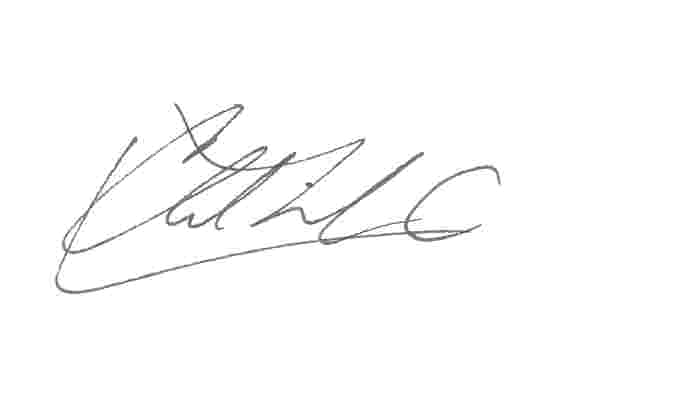
\includegraphics[scale=0.6]{firma.jpg}
 % \caption{}
  \label{fig:firma}
\end{center}
\end{figure}
\end{document} 